\documentclass{article}
\title{Inferring generation-interval distributions from contact tracing data}
\author{Sang Woo Park, David Champredon and Jonathan Dushoff}

\usepackage{graphics}
\usepackage{adjustbox}

\usepackage{amsthm}
\usepackage{amsmath}
\usepackage{amssymb}
\usepackage{amsfonts}

\usepackage{hyperref}
\usepackage{natbib}
\usepackage{hyperref}
\bibliographystyle{chicago}
\date{\today}

\usepackage{xspace}
\newcommand*{\ie}{i.e.\@\xspace}

\usepackage{color}

\newcommand{\Rx}[1]{\ensuremath{{\mathcal R}_{#1}}} 
\newcommand{\Ro}{\Rx{0}}
\newcommand{\RR}{\ensuremath{{\mathcal R}}}
\newcommand{\tsub}[2]{#1_{{\textrm{\tiny #2}}}}

\newcommand{\comment}[3]{\textcolor{#1}{\textbf{[#2: }\textsl{#3}\textbf{]}}}
\newcommand{\jd}[1]{\comment{cyan}{JD}{#1}}
\newcommand{\swp}[1]{\comment{magenta}{SWP}{#1}}
\newcommand{\dc}[1]{\comment{blue}{DC}{#1}}
\newcommand{\hotcomment}[1]{\comment{red}{HOT}{#1}}

\begin{document}
\maketitle

\section{Introduction}

An epidemic can be characterized by its speed (exponential growth rate, $r$) and its strength (reproductive number, \RR).
Reproductive number, defined as the average number of secondary cases arising from a primary case, is of particular interest as it provides information about the final size of an epidemic [CITE].
However, directly measuring the reproductive number often requires detailed knowledge of disease natural history and may not be feasible early in an epidemic [CITE].
Instead, the reproductive number can be \emph{indirectly} estimated from exponential growth rate, which can easily be estimated from incidence data [CITE].
These two quantities are linked by generation-interval distributions \citep{wallinga2007generation}.

Generation interval is defined as the time between when a person becomes infected and when that person infects another person.
Due to individual variation in infection time, the observed generation-interval distribution can change depending on when and how it is measured \citep{svensson2007note, kenah2008generation, nishiura2010time}.
There are important distinctions to be made when estimating generation intervals: \emph{intrinsic} generation intervals are measured by evaluating the infectiousness of infected people,
%% without regard to actual infection events,
while \emph{observed} generation intervals refer to the time between actual infection events.
Observed generation intervals in turn can be \emph{aggregated} across time, measured \emph{forward} in time by looking at a cohort of individuals infected at the same time and asking when they infected others, or measured \emph{backward in time} by look at a cohort and asking when their infectors were infected \citep{champredon2015intrinsic}.
% When aggregated generation intervals are observed until a given time in an ongoing epidemic (often via contact tracing), we refer to these as \emph{censored} (or right-censored) intervals.

Early in the epidemic when depletion of susceptible is negligible, we expect the forward generation-interval distribution to be similar to the intrinsic generation-interval distribution.
As epidemic progresses, an infector is less likely to infect individuals later in time due to decrease in susceptibles and the distribution of forward generation intervals will be shorter than the intrinsic distribution.
Conversely, when an epidemic is growing exponentially, as often occurs near the beginning of an outbreak, the number of newly infected individuals will be large relative to the number infected earlier on. 
A susceptible individual is thus relatively more likely to be infected by a newly infected individual, and the distribution of backward generation intervals will be shorter than the intrinsic distribution.
When epidemic is subsiding, most infections are caused by the remaining infectors, rather than new infectors, and the backward generation interval will be long.
\swp{Where can I cite champredon? First sentence? Last sentence? Or don't cite DC because I already did in the previous paragraph?}

In practice, generation intervals are measured by contact tracing throughout the course of an epidemic, usually aggregated to increase the amount of information available; we refer to these as \emph{censored} (or right-censored) intervals.
\jd{I kind of feel like, if you go on forever, aggregated GIs approach intrinsic GIs. This obviously isn't true for a single epidemic (observed GIs are shorter overall). On the other hand, it obviously \emph{is} true if you add births and get to a stable equilibrium. So I guess the remaining question is, do we get convergence if we have stable cycles? What we think about this will affect how we write the rest of this P.} \swp{Going to leave this comment here so that we can come back later.}
If observation goes on throughout the disease cycle, then (something about something).
On the other hand, if calculations are being done based on early-outbreak data, the available censored data is best thought of as a weighted average of backward generation-interval distributions; like them, the observed censored intervals will be shorter than intrinsic distributions.

Aggregating generation intervals across heterogeneous environment also affects the observed generation intervals.
Infection is more likely to spread quicker than on average among closely related inidividuals, and the local decrease in susceptibles result in shorter realized generation intervals.
\cite{trapman2016inferring} gave a similar argument to explain the difference in the the reproductive numbers between a homogeneously mixing population and a heterogeneously (network structured) mixing population.
Their result can be interpreted as a consequence of changes in generation-interval distributions: shorter generation intervals lead to smaller reproductive number [CITE]. 

\swp{Will rewrite this paragraph after writing the rest of it:}
In this study, we explore the temporal and spatial variation in the observed generation-interval distributions obtained from contact tracing.
We show that using the observed generation-interval distribution directly will always underestimate the reproductive number \swp{need to confirm this statement when we're done with the ms}. 
We provide a statistical framework of recovering the intrinsic generation-interval distribution from the observed generation-interval distribution.

\swp{Going to rename the sections... but I think I like the current order...}
\section{Generation-interval distributions across time}

We begin by introducing an analytical framework.
Let $K_a(\tau)$ be an individual level kernel, i.e., the rate at which secondary infections are caused by an individual $a$ \citep{svensson2015influence}. \swp{Need to say something more about Sven; come back later}
Then, the unconditional, population-level kernel is given by integrating over individual variations:
\begin{equation}
K(\tau) = \int K_a (\tau) dA.
\end{equation}
The basic reproductive number -- average number of secondary cases caused by an average primary case in a fully susceptible population -- is defined as: 
\begin{equation}
\RR_0 = \int K(t).
\end{equation}
Then, the intrinsic generation-interval is simply the population-level kernel normalized by the basic reproductive number:
\begin{equation}
g(\tau) = \frac{K(t)}{\RR_0}.
\end{equation}
Finally, the renewal equation model can be used to model incidence over time:
\begin{equation}
i(\tau) = S(\tau) \int K(s) i(\tau-s) ds = \RR S(\tau) \int g(s) i(\tau-s) ds
\end{equation}
where $i(\tau)$ is incidence at time $\tau$ and $S(\tau)$ is the proportion of the population susceptible.

\subsection*{Right-censored interval}

Assume that contact tracing is performed from the beginning of an epidemic to time $t$.
The number of infection occuring at time $s$ caused by infectors who were themselves infected at time $s-\tau$ is given by
\begin{equation}
i_{s-\tau}(s) = \RR i(s-\tau) g(\tau) S(s)
\end{equation}
Then, total number of secondary infections that are $\tau$ time steps apart and occur before time $t$:
\begin{equation}
\RR \int_\tau^t i(s-\tau) g(\tau) S(s) ds.
\end{equation}
Then, the censored interval at time $t$ is given by
\begin{equation}
c_t(\tau)= \frac{\RR \int_\tau^t i(s-\tau) g(\tau) S(s) ds}{\RR \int_0^t \int_x^t i(s-x) g(x) S(s) ds dx}.
\end{equation}
We note that the expression in the denominater is equivalent to cumulative incidence at time $t$.
The intuition behind this is that we are normalizing acrosss all incidence before time $t$.
Then, we have
\begin{equation}
c_t(\tau) = \frac{\RR \int_\tau^t i(s-\tau) g(\tau) S(s) ds}{\int_0^t i(s) ds}.
\end{equation}
For convenience, we ignore normalizing constants and write
\begin{equation}\label{eq:obsg}
c_t(\tau) \propto g(\tau) \int_{0}^t i(s-\tau) S(s) ds.
\end{equation}

For a single epidemic, the observed mean generation interval through contact tracing will always be shorter than intrinsic mean generation interval (Figure~\ref{fig:censor}).
There are two reasons for this phenomenon.
First, any infection events that occur after the contact tracing period canonot be observed due to right censoring and the observed generation-interval will be shorter.
In particular, when an epidemic is growing exponentially ($i(t) \propto \exp(rt)$), 
the censored generation-interval distribution is equivalent to the inverse exponentially weighted intrisnc generation-interval distribution:
\begin{equation}
\tsub{c}{exp}(\tau) \propto g(\tau) \exp(-r\tau).
\end{equation}
As backward generation-interval distributions are always shorter than the intrinsic generation-interval distribution during the exponential growth period, their weighted average (i.e., the censored intervals) will also be shorter.

Second, number of susceptibles decrease over the course of an epidemic, forward generation-interval distribution at any given period is always shorter than the intrinsic distribution \citep{champredon2015intrinsic}.
Asymptotically, we can ignore the effect of right-censoring, and the censored generation intervals can be thought of as a weighted average of the forward generation intervals.
As a result, even if contact tracing is performed through an entire epidemic, mean generation interval will be underestimated.

\begin{figure}
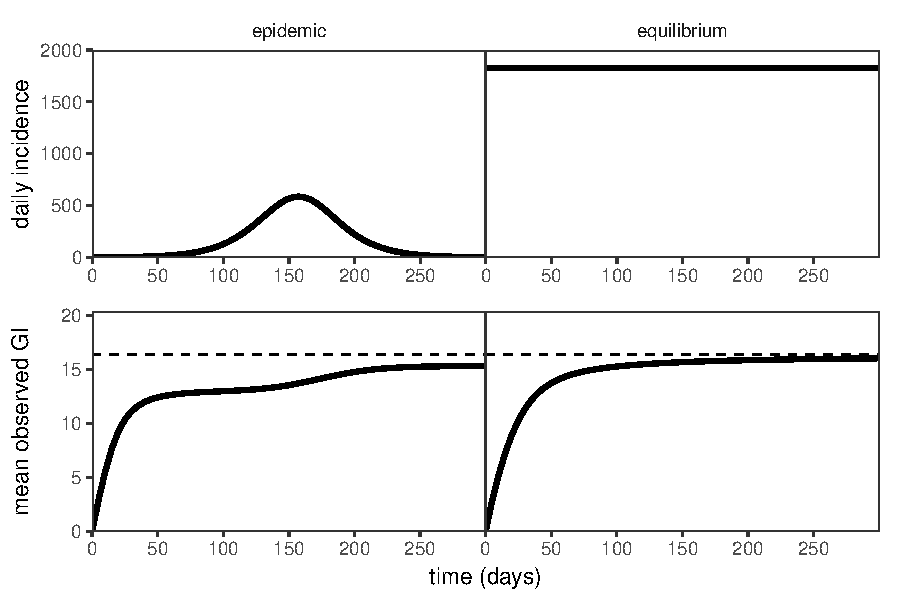
\includegraphics[width=\textwidth]{../analysis/temporal_effect.pdf}
\caption{Fill this out.}
\label{fig:censor}
\end{figure}

When an epidemic is in an equilibrium state (i.e., incidence $i(t)$ and the number of susceptibles $S(t)$ is constant over time), the observed generation-interval distribution is equivalent to the intrinsic generation-interval distribution.
On the other hand, when an epidemic is in a cycle, we get ???  \swp{TODO: Continue this exciting research!}

\section{Generation-interval distributions across space}

\subsection*{Conditional kernel}

Given limited contact structure, a susceptible individual can be contacted multiple times;
infectious contacts give rise to infection only when the susceptible individual is contacted for the first time.
Then, the conditional kernel (conditional on the infection occuring) of an individual $a$ is given by
\begin{equation}
\hat{k}_a(\tau) = k_a(\tau) \exp \left(- \delta_a \int_0^\tau k_a(s) ds\right),
\end{equation}
where $\delta_a$ is the dilution.
The individual kernel, $k_a(s)$, measures the intrinsic infectiousness of an individual $a$,
whereas $\delta_a k_a(s)$ measures the infectiousness of an individual $a$ for a particular susceptible individual.
Then, the population-level conditional kernel is:
\begin{equation}
\hat{k}(\tau) = \int \hat{k}_a(\tau) dA,
\end{equation}
and the conditional generation-interval distribution, defined to be the distribution of times at which secondary infections occur from a single primary infector, is:
\begin{equation}
\hat{g}(\tau) = \frac{\hat{k}(\tau)}{\int \hat{k} \tau}.
\end{equation}
\swp{Need to say something about trapman!!! Maybe say this is a generalization of Trapman's work...? Is that too much?}

The difference between conditional and intrinsic generation-interval distribution can be best demonstrated by simulating stochastic infection processes on a small tree network -- a single infected individual is connected to multiple susceptible individuals but susceptibles are not connected with each other -- with artificially high $\RR$ (Figure ??? to be made).
We observe that the distribution of realized generation times matches with the conditional generation-interval distribution, whereas the distribution of contact times matches with the intrinsic generation-interval distribution.
On the other hand, if a stochastic infection processes are simulated on a small homogeneous network with all else being equal, the distribution of generation times is even shorter than the effective generation intervals because a susceptible individual may be contacted by multiple infectors (and only the first contact gives rise to infection).
\jd{Let's think about how to explain this. In particular, the first one is where we have our correction that works \ldots}.
Hence, we expect there to be varying degrees of local depletion of susceptibles in a heterogeneous contact structure and the accurate measurement of generation interval will be more difficult.

\section{Statistical approach to estimating generation-interval distribution}

The observed generation-interval distribution is a weighted intrinsic generation-interval distribution (equation~\ref{eq:obsg}),
Then, the intrinsic generation interval can be recovered by taking the inverse weights:
\begin{equation}
g(\tau) \propto g_t(\tau) \frac{1}{\int_{0}^t i(s-\tau) S(s) ds}
\end{equation}
However, this method requires a knowledge of susceptible dynamics and may not be feasible in practice.

During exponential growth period, we can write $i(\tau) \propto \exp(r t)$, where $r$ is the exponential growth rate.
Assuming that $S(t) \approx 1$, the observed generation-interval distribution during growth period can be written as follows:
\begin{equation}
\tsub{g}{exp}(\tau) \propto g(\tau) \exp(-r\tau),
\end{equation}
Taking the inverse weight, we obtain the following expression for the intrinsic generation-interval distribution:
\begin{equation}
g(\tau) \propto \tsub{g}{exp}(\tau) \exp(r\tau)
\end{equation}
and the reproductive number:
\begin{equation}
\RR = \int_0^\infty \tsub{g}{exp}(\tau) \exp(r\tau) d\tau.
\end{equation}
Therefore, applying the Lotka-Euler equation using the observed generation interval via contact tracing results in underestimation of reproductive number:
\begin{equation}
\int_0^\infty \tsub{g}{exp}(\tau) \exp(r\tau) d\tau > \left(\int_0^\infty \tsub{g}{exp}(\tau) \exp(-r\tau) d\tau\right)^{-1}
\end{equation}
This method provides a non-parametric approach for inferring the intrinsic generation-interval distribution and the reproductive number from contact tracing data.

\swp{Need to rewrite this section. It's merely a place holder for now:}
While the non-parametric method is simple, it does not use all available information from contact tracing data.
In particular, it does not take into account who infected whom.
Assuming a poisson process, we can obtain a likelihood for observing infections:
\begin{equation}
\RR^{n_e} \cdot \prod g(\tau_e) \cdot \exp \left(- \RR \int_0^{c - t_{\tiny\textrm{inf}}} g(s) ds \right)
\end{equation}
This method requires us to make an assumption about the generation-interval distributions... See example...




\section{Methods}



\bibliography{network}
\end{document}
